\begin{figure*}[!htbp]
\begin{minipage}{6in}
\begin{center}

\begin{minipage}{\linewidth}
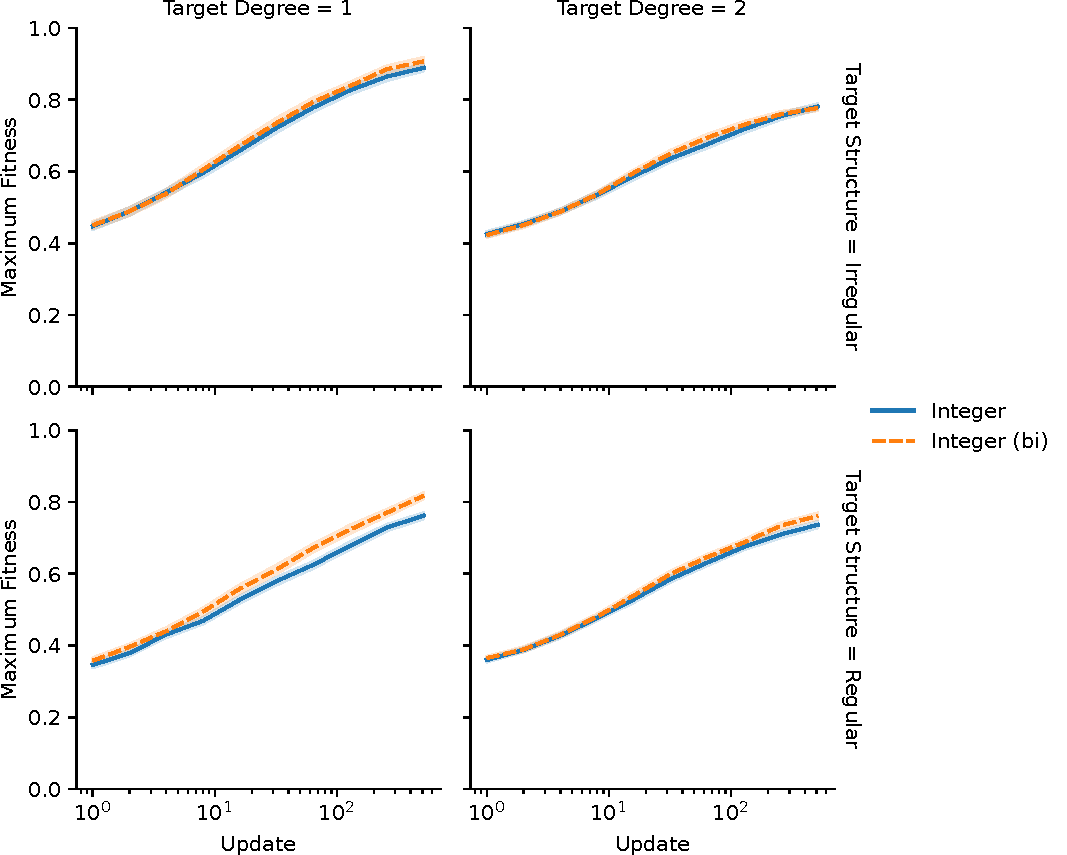
\includegraphics[width=\linewidth]{img/target_evolve_norm/viz=max-fitness-line+_data_hathash_hash=3e06b14c923ee265+_script_fullcat_hash=c26c8688c31571c2+ext=}
\end{minipage}
\begin{minipage}{\linewidth}
\caption{
Trajectories of adaptive evolution for each tag-matching metric on the 32-node graph-matching task with normally-distributed mutation.
Maximum fitness is the best fitness value for any individual within a population.
Reported results use each metric's best-performing standard deviation mutation rate.
(See Supplementary Figure \ref{fig:evolve_norm_mutsweep} for survey showing how mutation rate affects adaptive evolution under each metric.)
Note log-scale x-axes.
Shaded area represents bootstrapped 95\% confidence intervals across 50 replicate observations.
}
\label{fig:evolve_bests_norm}
\end{minipage}
\end{center}
\end{minipage}
\end{figure*}
